\documentclass{standalone}
\usepackage{tikz}
\usepackage{amsmath}
\renewcommand{\familydefault}{\sfdefault}
\usetikzlibrary{calc}

\begin{document}
% \begin{equation}
    % p(y = c | \mathbf{x}) \propto p(y=c) p(\mathbf{x} | y = c)
% \end{equation}
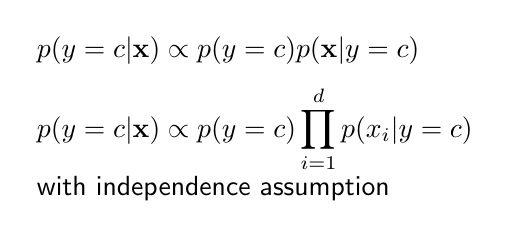
\begin{tikzpicture}  
    \node [anchor = west] at (0, 0) {$p(y = c | \mathbf{x}) \propto p(y=c) p(\mathbf{x} | y = c)$};
    \node [anchor = west] at (0, -1) {$\displaystyle p(y = c | \mathbf{x}) \propto p(y=c) \prod_{i=1}^d p(x_i | y = c)$};

    \node [anchor = west] at (0, -1.75) {with independence assumption};
\end{tikzpicture}    
\end{document}

